\chapter{The sensitivity of NOGWs excited by tropopause depressions}
\label{sec:resultsQ3D}


\begin{tcolorbox}[]
    (R1) How sensitive are NOGWs from propagating tropopause folds to the 2D shape of the depression and the stratospheric environment?
\end{tcolorbox}


% define quasi 3d simulations
Following the results of the model validation / comparison of GWD with linear solutions




\section{Quasi-3D reference Simulation}
\label{sec:resultsq3D-reference}


For the stratosphere the assumption of a two atomic gas  possible to de
\begin{figure*}[tbp]
    \centering
    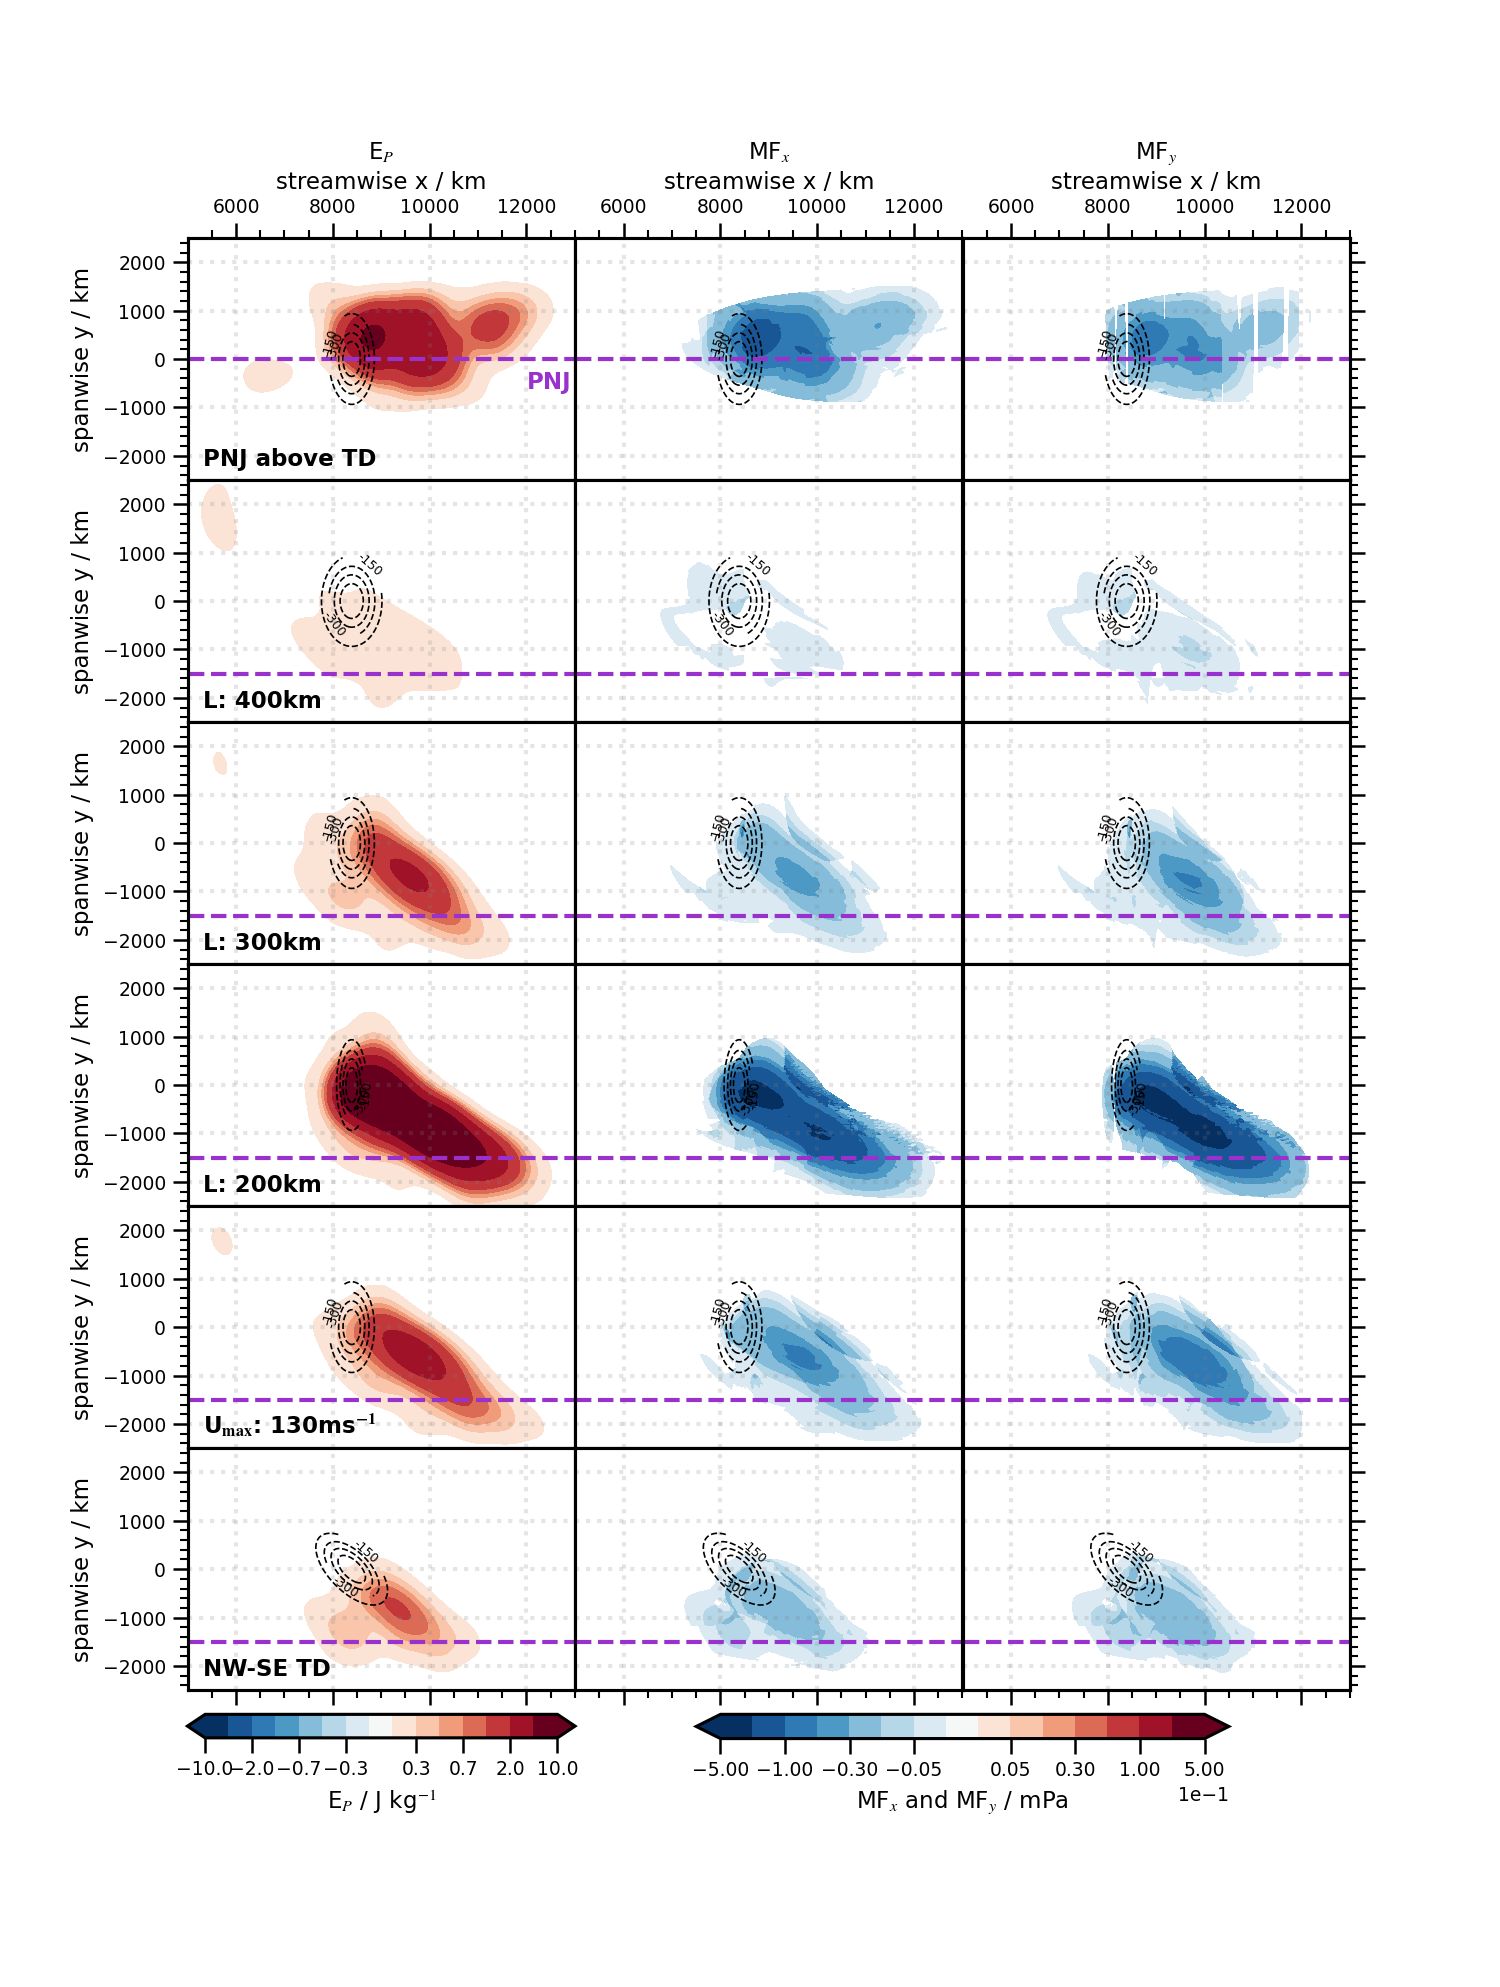
\includegraphics[width=0.99\textwidth]{figures_3D/waveletAna_fluxes_obs.png}
    \caption{Horizontal cross sections at 40km above the tropopause for five simulations with horizontal and meridional shear in a barotropic environment. Shown are $\theta$', $\lambda_x$ and $\lambda_y$ at 72h into the simulation. Dominant zonal and meridional wavelengths for each grid point are determined from wavelet analysis.}
    % \label{fig:waveletAna_dudy}
\end{figure*}

\section{Influence of tropopause shape}

\section{Influence of background zonal wind ambient}

\section{Influence of Coriolis force and stratification}

\section{Influence of tropopause speed / propagation}

show constant wind simulations + normal ones!!

comparison of MFx and so on or not?

\section{Summary and answer to research question (R1)}

\begin{tcolorbox}[]
    (R1) How sensitive are NOGWs from propagating tropopause folds to the 2D shape of the depression and the stratospheric environment?
\end{tcolorbox}